% Generated by render.py; edit preamble.tex, citations.json and connections.tikz
\documentclass[border=12pt]{standalone}
\def\pgfsysdriver{pgfsys-dvisvgm.def}
\usepackage[dvisvgm]{xcolor}
\usepackage{xeCJK}
\setCJKmainfont{HaranoAjiGothic-Regular.otf}[BoldFont=HaranoAjiGothic-Bold.otf]
\setCJKsansfont{HaranoAjiGothic-Regular.otf}[BoldFont=HaranoAjiGothic-Bold.otf]
\usepackage{amsmath,amssymb,tikz,lmodern}
\usetikzlibrary{arrows.meta,positioning,calc,fit,backgrounds}
\renewcommand{\familydefault}{\sfdefault}
\definecolor{ink}{HTML}{25322F}
\definecolor{green}{HTML}{246657}
\definecolor{tint}{HTML}{EEF4F0}
\definecolor{soft}{HTML}{C6D2CC}
\definecolor{muted}{HTML}{52615B}
\newif\ifJapanese
\newcommand{\Tx}[2]{\ifJapanese #1\else #2\fi}
\newcommand{\Eff}{\overline{\operatorname{Eff}}}
\newcommand{\heading}[3]{{\color{green}\bfseries #1\quad\Tx{#2}{#3}}\\[5pt]}
% A white rectangle makes the complete citation label clickable, including spaces.
\newcommand{\refurl}[2]{\special{dvisvgm:raw <a xlink:href="#1" target="_blank" rel="noopener noreferrer">}{\setlength{\fboxsep}{0pt}\colorbox{white}{\color{green}\underline{\strut #2}}}\special{dvisvgm:raw </a>}}
\tikzset{
 card/.style={draw=soft,fill=white,rounded corners=2pt,align=left,text=ink,font=\fontsize{10.5}{14}\selectfont,inner xsep=12pt,inner ysep=10pt,text width=14.4cm},
 half/.style={card,text width=6.45cm,minimum height=2.05cm},
 result/.style={card,draw=green,fill=tint,line width=.9pt},
 reason/.style={align=left,text=muted,font=\fontsize{9}{12}\selectfont,inner sep=0pt,text width=12.6cm},
 branchreason/.style={reason,text width=5.95cm},
 edge/.style={-{Stealth[length=2.4mm]},draw=green,line width=1pt},
 wire/.style={draw=green,line width=1pt},
}
% Keep the arrow in a dedicated left gutter; explanations never cover it.
\def\flow#1#2#3;{
 \coordinate (#2-from) at ($(#1.south)+(-6.9,0)$);
 \coordinate (#2-to) at ($(#2.north)+(-6.9,0)$);
 \draw[edge] (#2-from)--(#2-to);
 \node[reason,anchor=west] (#2-reason) at ($(#2-from)!.5!(#2-to)+(.55,0)$) {#3};
}

% Style adapted from the repository's Schnell diagrams; MIT attribution retained.

% Generated from citations.json; do not edit.
\newcommand{\Cite}[1]{\csname cite-#1\endcsname}
\expandafter\def\csname cite-tf-main\endcsname{\shortstack[l]{\refurl{https://github.com/openai/math/blob/1581d4cbdd69a0faf34b2089614fe2a814316a6a/preprints/A-Torsion-Free-Group-Algebra-That-Is-Not-Directly-Finite-October-4-2026/direct-finiteness.pdf}{[OpenAI26tf, Theorem 1.1, p. 1]}}}
\expandafter\def\csname cite-two-main\endcsname{\shortstack[l]{\refurl{https://github.com/openai/math/blob/1581d4cbdd69a0faf34b2089614fe2a814316a6a/preprints/A-Counterexample-to-Kaplanskys-Direct-Finiteness-Conjecture-in-Characteristic-Two-September-23-2026/paper.pdf}{[OpenAI26two, Theorem 1.1, p. 1]}}}
\expandafter\def\csname cite-two-ca\endcsname{\shortstack[l]{\refurl{https://github.com/openai/math/blob/1581d4cbdd69a0faf34b2089614fe2a814316a6a/preprints/A-Counterexample-to-Kaplanskys-Direct-Finiteness-Conjecture-in-Characteristic-Two-September-23-2026/paper.pdf}{[OpenAI26two, Corollary 7.3, p. 26]}}}
\expandafter\def\csname cite-det-input\endcsname{\shortstack[l]{\refurl{https://github.com/openai/math/blob/1581d4cbdd69a0faf34b2089614fe2a814316a6a/preprints/A-Counterexample-to-the-Group-Ring-Determinant-Conjecture-September-23-2026/paper.pdf}{[OpenAI26det, Theorem 1.2; §5, pp. 2, 8]}}}
\expandafter\def\csname cite-det-main\endcsname{\shortstack[l]{\refurl{https://github.com/openai/math/blob/1581d4cbdd69a0faf34b2089614fe2a814316a6a/preprints/A-Counterexample-to-the-Group-Ring-Determinant-Conjecture-September-23-2026/paper.pdf}{[OpenAI26det, Theorem 1.1, p. 2]}}}
\expandafter\def\csname cite-odd-main\endcsname{\shortstack[l]{\refurl{https://github.com/openai/math/blob/1581d4cbdd69a0faf34b2089614fe2a814316a6a/preprints/A-Counterexample-to-Kaplanskys-Direct-Finiteness-Conjecture-in-Odd-Characteristic-September-26-2026/paper.pdf}{[OpenAI26odd, Theorem 1.1, p. 1]}}}
\expandafter\def\csname cite-odd-ca\endcsname{\shortstack[l]{\refurl{https://github.com/openai/math/blob/1581d4cbdd69a0faf34b2089614fe2a814316a6a/preprints/A-Counterexample-to-Kaplanskys-Direct-Finiteness-Conjecture-in-Odd-Characteristic-September-26-2026/paper.pdf}{[OpenAI26odd, Proposition 8.1, p. 23]}}}
\expandafter\def\csname cite-es04\endcsname{\shortstack[l]{\refurl{https://arxiv.org/pdf/math/0305440v2\string##page=8}{[ES04, Corollary 4.7, p. 8]}}}
\expandafter\def\csname cite-es05\endcsname{\shortstack[l]{\refurl{https://arxiv.org/pdf/math/0408400v2\string##page=18}{[ES05, Theorem 5, p. 18]}}}
\expandafter\def\csname cite-overview\endcsname{\shortstack[l]{\refurl{https://github.com/openai/math/blob/1581d4cbdd69a0faf34b2089614fe2a814316a6a/overview.pdf}{OpenAI Research Catalog · Catalogue 197 / Algebra · p. 21}}}

\Japanesetrue
\begin{document}
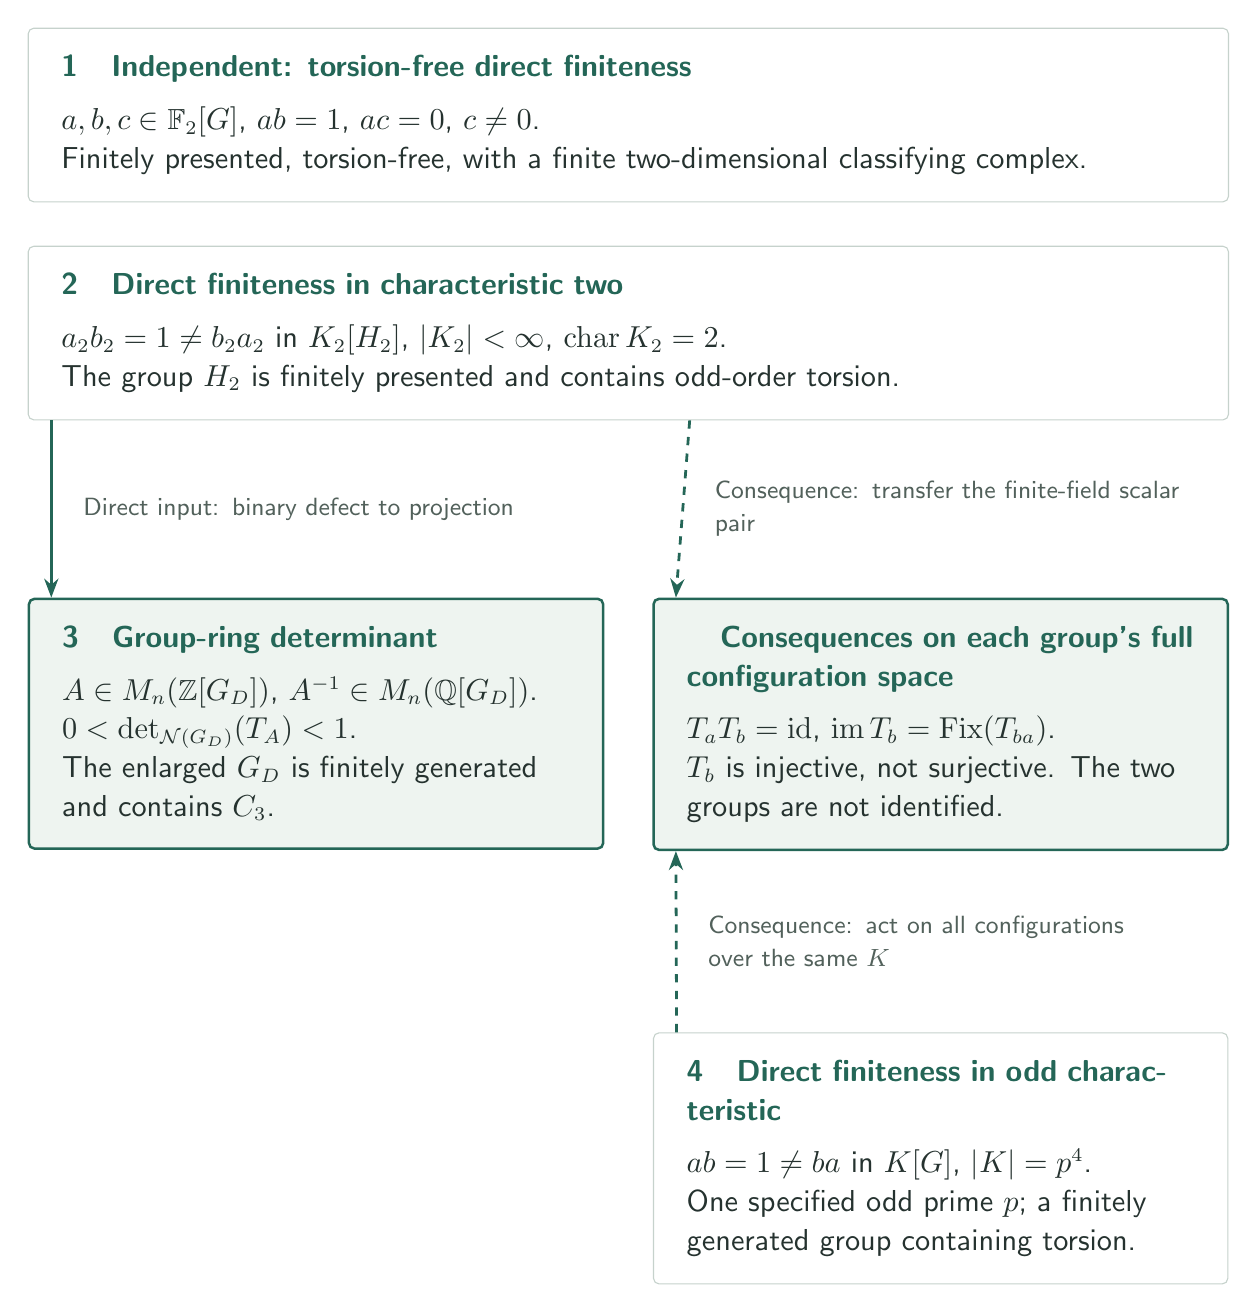
\begin{tikzpicture}
\node[card] (tf) {\heading{1}{独立構成：Torsion-free direct finiteness}{Independent: torsion-free direct finiteness}$a,b,c\in\mathbb F_2[G]$, $ab=1$, $ac=0$, $c\ne0$.\\\Tx{有限表示・torsion-free・有限2次元分類複体。}{Finitely presented, torsion-free, with a finite two-dimensional classifying complex.}\\\Cite{tf-main}};
\node[card,below=.55cm of tf] (two) {\heading{2}{Direct finiteness in characteristic two}{Direct finiteness in characteristic two}$a_2b_2=1\ne b_2a_2$ in $K_2[H_2]$, $|K_2|<\infty$, $\operatorname{char}K_2=2$.\\\Tx{$H_2$は有限表示で奇数位数のtorsionを含む。}{The group $H_2$ is finitely presented and contains odd-order torsion.}\\\Cite{two-main}};
\node[result,text width=6.45cm,minimum height=2.9cm,anchor=north west] (det) at ($(two.south west)+(0,-2.25)$) {\heading{3}{Group-ring determinant}{Group-ring determinant}$A\in M_n(\mathbb Z[G_D])$, $A^{-1}\in M_n(\mathbb Q[G_D])$.\\$0<\det_{\mathcal N(G_D)}(T_A)<1$.\\\Tx{拡大群$G_D$は有限生成、$C_3$を含む。}{The enlarged $G_D$ is finitely generated and contains $C_3$.}\\\Cite{det-main}};
\node[result,text width=6.45cm,minimum height=2.9cm,anchor=north east] (ca) at ($(two.south east)+(0,-2.25)$) {\heading{}{各構成群の全配置上の帰結}{Consequences on each group's full configuration space}$T_aT_b=\operatorname{id}$, $\operatorname{im}T_b=\operatorname{Fix}(T_{ba})$.\\\Tx{$T_b$は単射・非全射。二つの群を同一視しない。}{$T_b$ is injective, not surjective. The two groups are not identified.}};
\node[half,below=2.3cm of ca] (odd) {\heading{4}{Direct finiteness in odd characteristic}{Direct finiteness in odd characteristic}$ab=1\ne ba$ in $K[G]$, $|K|=p^4$.\\\Tx{一つの指定奇素数$p$、有限生成群、torsionを含む。}{One specified odd prime $p$; a finitely generated group containing torsion.}\\\Cite{odd-main}};
\coordinate (dstart) at ($(two.south west)+(.3,0)$);
\coordinate (dend) at ($(det.north west)+(.3,0)$);
\draw[edge] (dstart)--(dend);
\node[branchreason,anchor=west] at ($(dstart)!.5!(dend)+(.4,0)$) {\Tx{直接入力：二進欠損を射影へ}{Direct input: binary defect to projection}\\\Cite{det-input}};
\coordinate (cstart) at ($(two.south east)+(-6.85,0)$);
\coordinate (cend) at ($(ca.north west)+(.3,0)$);
\draw[edge,dashed] (cstart)--(cend);
\node[branchreason,anchor=west] at ($(cstart)!.5!(cend)+(.4,0)$) {\Tx{帰結：有限体のscalar対を移す}{Consequence: transfer the finite-field scalar pair}\\\Cite{two-ca}};
\coordinate (ostart) at ($(odd.north west)+(.3,0)$);
\coordinate (oend) at ($(ca.south west)+(.3,0)$);
\draw[edge,dashed] (ostart)--(oend);
\node[branchreason,anchor=west] at ($(ostart)!.5!(oend)+(.4,0)$) {\Tx{帰結：同じ$K$で全配置へ作用}{Consequence: act on all configurations over the same $K$}\\\Cite{odd-ca}};

\end{tikzpicture}
\end{document}
